\documentclass[a4paper,12pt]{article}
\usepackage[utf8]{inputenc}
\usepackage[T1]{fontenc}
\usepackage{geometry}
\usepackage{graphicx}
\usepackage{amsmath,amssymb}
\geometry{margin=2.5cm}

\begin{document}

\noindent\textbf{UDC 004.85}\\[2ex]
\begin{center}
  {\LARGE \textbf{Neural Networks Loss Landscape Convergence in Hessian Low-Dimensional Space}}\\[2ex]
  Tem Nikitin, Nikita Kiselev\\[1ex]
  Moscow Institute of Physics and Technology, Moscow, Russia
\end{center}
Understanding how a neural network’s loss landscape changes as we add more training data is important for efficient training. Although larger datasets reshape this high-dimensional surface, the point when extra data stop making a big difference is unclear. We show that near a local minimum the loss landscape stabilizes once the dataset exceeds a certain size. To study this, we project the full parameter space onto a lower-dimensional subspace formed by the Hessian’s top eigenvectors, highlighting the most important curvature directions. Within this subspace, we use Monte Carlo sampling to estimate how the loss changes more precisely. Experiments on standard image classification tasks demonstrate that our low-dimensional analysis pinpoints when the landscape stops evolving, offering practical guidance for balancing training cost with performance improvements.


\section*{Thesis}

Deep neural networks often improve when we feed them more data, because extra samples make the loss surface smoother and help the model generalize. But after a certain point, new data barely changes the local shape of the loss, and collecting more can waste time and resources. We need a way to find the minimal amount of data that still shapes the model’s behaviour well.

We offer a simple bound (Theorem~1) for the average squared change in loss:
$$
\Delta_k = \mathbb{E}[L_{k+1}(w) - L_k(w)]^2 \approx \frac{\sigma^4}{4} \Bigl(2\sum_{d=1}^D(\lambda_{k+1}^{(d)} - \lambda_k^{(d)})^2 + \bigl(\sum_{d=1}^D(\lambda_{k+1}^{(d)} - \lambda_k^{(d)})\bigr)^2\Bigr),
$$
where $\lambda_k^{(d)}$ are the top $D$ eigenvalues of the Hessian at batch size $k$, and $\sigma^2$ measures random perturbations. This formula works in a low-dimensional space spanned by the main curvature directions.

Our method runs as follows:
\begin{itemize}
  \item Use power iterations to find the top $D=10$ Hessian eigenvectors.
  \item After each new mini-batch, project updates onto this subspace and compute both the actual $\Delta_k$ by sampling and the bound above.
  \item Stop adding data once the bound drops below a chosen tolerance $\Delta$.
\end{itemize}

We tested on MNIST and Fashion-MNIST with simple MLP and CNN models. Figure~\ref{fig:delta} shows that the 
theoretical bound stays above the measured $\Delta_k$ curves and shrinks roughly like $O(1/k^2)$. Table~1 lists the minimal batch sizes $K$ needed for tolerances of 0.025 and 0.030. Values range from 40 to 120, and more complex models converge faster because they capture sharper directions.

Each step costs $O(I\,D\,C_{Hv})$ operations, where $I$ is power-iteration steps and $C_{Hv}$ is the cost of a Hessian-vector product. We also discuss simple tricks, like reducing $D$ or stopping iterations early, to speed this up.

In future work, we plan to apply this to deeper, non-convex networks, data streams, and active sampling. Embedding this check in online learning could let systems decide in real time whether to ask for more data.

\begin{figure}[ht]
  \centering
  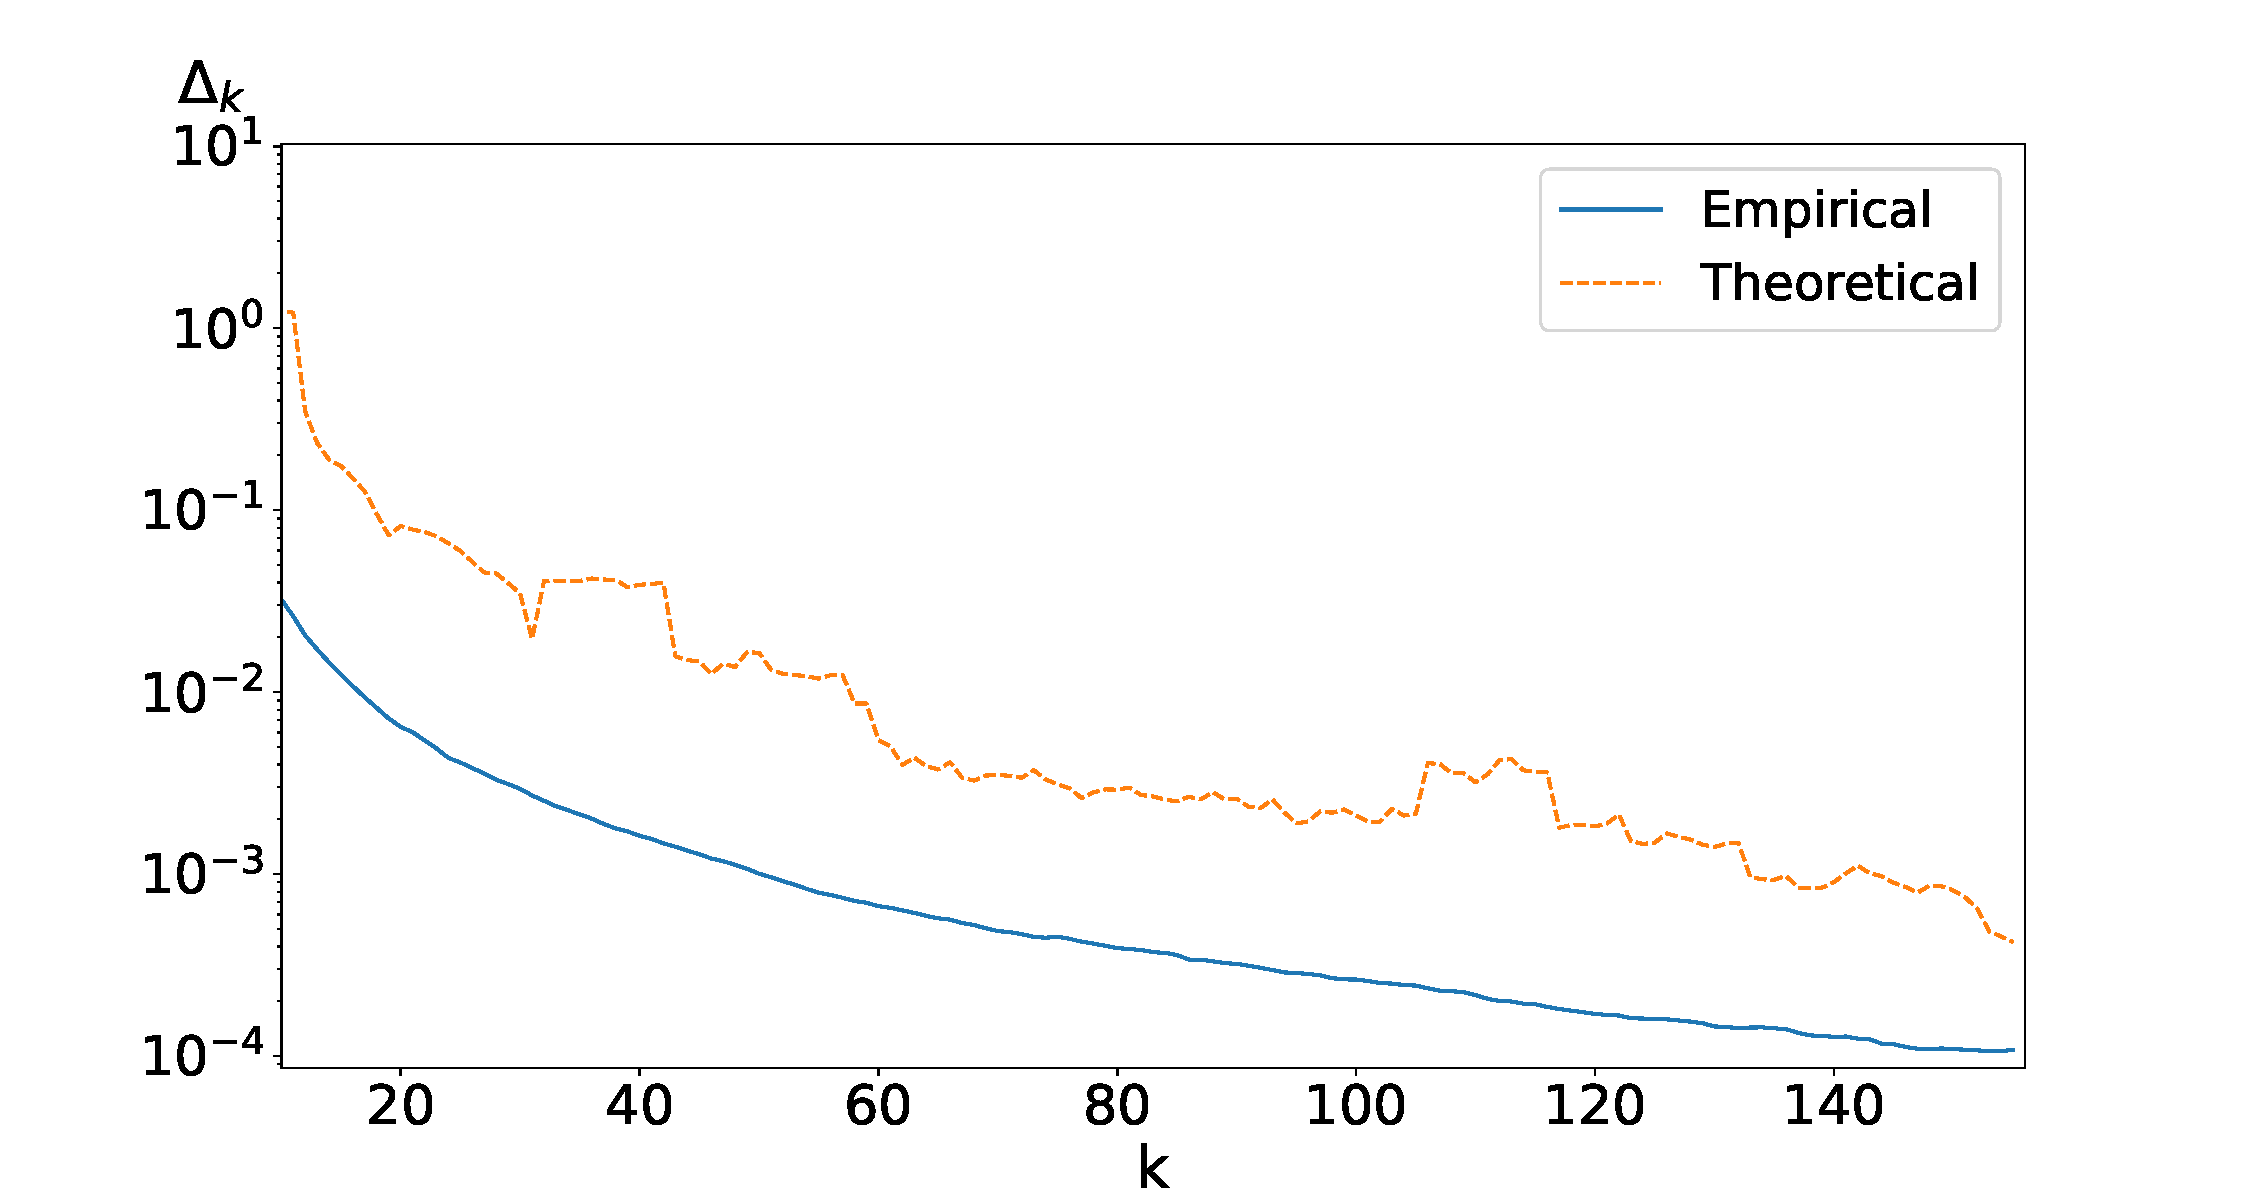
\includegraphics[width=0.8\textwidth]{img/delta_border_1_10_1024.pdf}
  \caption{Empirical and theoretical $\Delta_k$ for MNIST experiments.}
  \label{fig:delta}
\end{figure}

\begin{table}[ht]
  \centering
  \caption{$\Delta$-sufficient sample size results}
  \begin{tabular}{lccc}
    \hline
    Dataset & Model & $\Delta$ & $K$ \\
    \hline
    MNIST & Single-layer MLP & 0.025 & 100 \\
    MNIST & Convolutional CNN & 0.025 & 60 \\
    Fashion-MNIST & CNN & 0.030 & 70 \\
    \hline
  \end{tabular}
\end{table}

\paragraph{Funding and Acknowledgements}
This work was supported by the Moscow Institute of Physics and Technology. We thank the HPC Center for computing resources and helpful discussions on Hessian analysis.

\begin{thebibliography}{9}
  \bibitem{soy2020} D. Soydaner, \textit{A comparison of optimization algorithms for deep learning}, Int. J. Pattern Recognit. Artif. Intell., 34(13):2052013, 2020.
  \bibitem{wu2017} L. Wu, Z. Zhu, W. E., \textit{Towards understanding generalization of deep learning: Perspective of loss landscapes}, arXiv:1706.10239, 2017.
  \bibitem{cookbook} K. B. Petersen, M. S. Pedersen, \textit{The Matrix Cookbook}, 2012.
  \bibitem{deng2012} L. Deng, \textit{The MNIST database of handwritten digit images for machine learning research}, IEEE Signal Process. Mag., 29(6), 2012.
  \bibitem{xiao2017} H. Xiao, K. Rasul, R. Vollgraf, \textit{Fashion-MNIST: a novel image dataset for benchmarking machine learning algorithms}, arXiv:1708.07747, 2017.
\end{thebibliography}

\end{document}